\chapter{Cài đặt công cụ và thực nghiệm}\label{chap4}
\section{Công cụ thực nghiệm}
Nhằm đánh giá tính hiệu quả của phương pháp đề xuất, khóa luận đã cài đặt một số mô-đun và tích hợp phương pháp đề xuất trên công cụ AKAUTAUTO và thực hiện thực nghiệm trên công cụ này. AKAUTAUTO là một công cụ kiểm thử tự động cho mã nguồn C/C++, được nghiên cứu và phát triển bởi Phòng thí nghiệm Đảm bảo chất lượng phần mềm (Khoa Công nghệ thông tin, Trường Đại học Công nghệ, ĐHQGHN) và đơn vị FPT-GAM (FPT Global Automative \& Manufacturing). Khóa luận kế thừa kiến trúc của công cụ AKAUTAUTO phiên bản 5.9.2, phiên bản tích hợp sẵn phương pháp kiểm thử tượng trưng động và phương pháp sinh giả lập mã nguồn tự động AS4UT, và bổ sung, cải tiến một số mô-đun trong kiến trúc gốc để tích hợp phương pháp đề xuất (phiên bản 5.9.2-thesis).

\subsection{Tổng quan kiến trúc công cụ AKAUTAUTO}
Công cụ AKUTAUTO được phát triển bằng ngôn ngữ Java với kiến trúc bao gồm sáu mô-đun chính lần lượt là mô-đun xây dựng môi trường kiểm thử, mô-đun phân tích mã nguồn, mô-đun xử lý hàm thiếu định nghĩa, mô-đun sinh dữ liệu kiểm thử, mô-đun thực thi \& phân tích ca kiểm thử và mô-đun sinh báo cáo kiểm thử. Hình \ref{fig:architect} mô tả kiến trúc của công cụ AKAUTAUTO gồm sáu mô-đun kể trên và các thành phần ngoài gồm trình biên dịch C/C++, bộ giải Z3 và thư viện phân tích mã nguồn CDT Parser. Trong đó, khóa luận đã bổ sung mô-đun xử lý hàm thiếu định nghĩa so với kiến trúc gốc, và cải tiến hai mô-đun phân tích mã nguồn và mô-đun sinh dữ liệu kiểm thử (thể hiện bởi các khối in đậm).

\begin{figure}[t]
    \centering
    \includesvg[width=\linewidth]{images/architect.svg}
    \caption{Kiến trúc công cụ AKAUTAUTO.}
    \label{fig:architect}
\end{figure}

Đầu vào của công cụ AKAUTAUTO gồm hai thành phần chính lần lượt là các tệp mã nguồn kiểm thử và cấu hình kiểm thử. Hai thành phần này được cung cấp bởi kiểm thử viên hoặc lập trình viên. Mô-đun xây dựng môi trường kiểm thử là mô-đun tiếp nhận các thành phần đầu vào và đảm nhiệm vai trò thực hiện hai tác vụ tiền xử lý mã nguồn trong pha xây dựng môi trường kiểm thử. Hai tác vụ tiền xử lý đã được đề cập ở Mục~\ref{sec:3-build-env} gồm thiết lập môi trường và tạo môi trường tính toán độ phủ. Mô-đun xây dựng môi trường kiểm thử cấu thành bởi ba thành phần chính đó là thành phần thiết lập môi trường, thành phần tải dự án và thành phần tạo môi trường tính toán độ phủ. Trong đó, hai thành phần thiết lập môi trường và tạo môi trường tính toán độ phủ thực hiện hai tác vụ tương ứng đã nêu. Thành phần tải dự án có nhiệm vụ xác định các tệp mã nguồn được người dùng thiết lập, sau đó kiến tạo đỉnh tệp của từng cây cấu trúc tệp tương ứng. Đầu ra của mô-đun gồm các tệp mã nguồn đã được thêm lệnh đánh dấu và tập các cây cấu trúc tệp cơ bản sinh bởi thành phần tải dự án. Các tệp mã nguồn chứa lệnh đánh dấu sẽ được sử dụng bởi mô-đun xử lý hàm thiếu định nghĩa nhằm sinh thân hàm giả trên tệp mã nguồn này. Tập cây cấu trúc tệp cơ bản và mã nguồn gốc sẽ được phân tích bởi mô-đun phân tích mã nguồn.

Các mô-đun tiếp theo trong kiến trúc của công cụ AKAUTAUTO được khóa luận bổ sung hoặc cải tiến gồm mô-đun phân tích mã nguồn, mô-đun xử lý hàm thiếu định nghĩa và mô-đun sinh dữ liệu kiểm thử. Chi tiết về sự cải tiến của mô-đun phân tích mã nguồn và mô-đun sinh dữ liệu kiểm thử được trình bày lần lượt ở Mục~\ref{sec:module-analyze} và Mục~\ref{sec:module-autogen}. Mô-đun xử lý hàm thiếu định nghĩa được bổ sung so với kiến trúc gốc nhằm giải quyết các vấn đề phát sinh bởi nguyên mẫu hàm thiếu định nghĩa. Nội dung chi tiết của mô-đun này được trình bày ở Mục~\ref{sec:module-undef}. 

Khóa luận kế thừa mô-đun thực thi và phân tích ca kiểm thử từ kiến trúc gốc của công cụ. Mô-đun này đóng vai trò  sinh trình điều khiển kiểm thử, thực thi trình điều khiển và phân tích đường thi hành thu được sau khi chạy ca kiểm thử. Cấu trúc của mô-đun gồm ba thành phần chính với nhiệm vụ chi tiết của từng thành phần như sau:
\begin{itemize}
    \item Thành phần sinh trình điều khiển kiểm thử: Đảm nhiệm hai vai trò chuyển đổi bộ nghiệm giải từ ràng buộc thành dữ liệu kiểm thử C++ và sinh trình điều khiển kiểm thử dựa trên dữ liệu mới. Trình điều khiển kiểm thử là một tệp C++ được tự động sinh ra nhằm chuyển đổi dữ liệu kiểm thử C++ thành các cú pháp C++ giúp khởi tạo giá trị tham số đầu vào của đơn vị kiểm thử. Các cú pháp C++ trong trình điều khiển gồm hai phần chính đó là phần định nghĩa tham số đầu vào và phần gọi đơn vị kiểm thử. Trình điều khiển cũng đảm nhiệm chuyển hóa dữ liệu kiểm thử C++ thành các mã nguồn giả lập cho các hàm cần stub.
    \item Thành phần thực thi ca kiểm thử: Có nhiệm vụ biên dịch trình điều khiển và các tệp mã nguồn chứa lệnh đánh dấu thành tệp đối tượng rồi sau đó liên kết các tệp này để tạo thành tệp thực thi. Công cụ chạy tệp thực thi này và thu được danh sách các câu lệnh, các nhánh điều kiện được viếng thăm bởi ca kiểm thử.
    \item Thành phần phân tích đường thi hành: Có chức năng ánh xạ danh sách các câu lệnh, nhánh điều kiện được viếng thăm sang đỉnh tương ứng trong CFG của đơn vị kiểm thử. Tiếp đó, thành phần cập nhật dữ liệu viếng thăm của CFG dựa trên tập đỉnh được ánh xạ. Cuối cùng, thành phần phân tích đường thi hành sẽ tìm đường thi hành ngắn nhất chưa được viếng thăm và truyền đường thi hành này sang mô-đun sinh dữ liệu kiểm thử.
\end{itemize}

Mô-đun cuối cùng trong kiến trúc công cụ là mô-đun sinh báo cáo kiểm thử. Mô-đun này có vai trò tính toán độ phủ của đơn vị kiểm thử dựa trên dữ liệu viếng thăm của CFG và tạo báo cáo kiểm thử sau khi quá trình sinh dữ liệu kiểm thử tự động kết thúc. Hình \ref{fig:report} mô tả ví dụ báo cáo kiểm thử LCOV của hàm \tcode{foo}. Khóa luận đã sinh dữ liệu kiểm thử tự động cho hàm \tcode{foo} và đạt được độ phủ 100\% câu lệnh cũng như 100\% nhánh với ba ca kiểm thử. Các thông tin ở góc trên phải của báo cáo cho biết 7/20 dòng lệnh của tệp chứa hàm \tcode{foo} và 4/4 nhánh điều kiện có trong hàm được thăm bởi ba ca kiểm thử này. 

\begin{figure}[h]
    \centering
    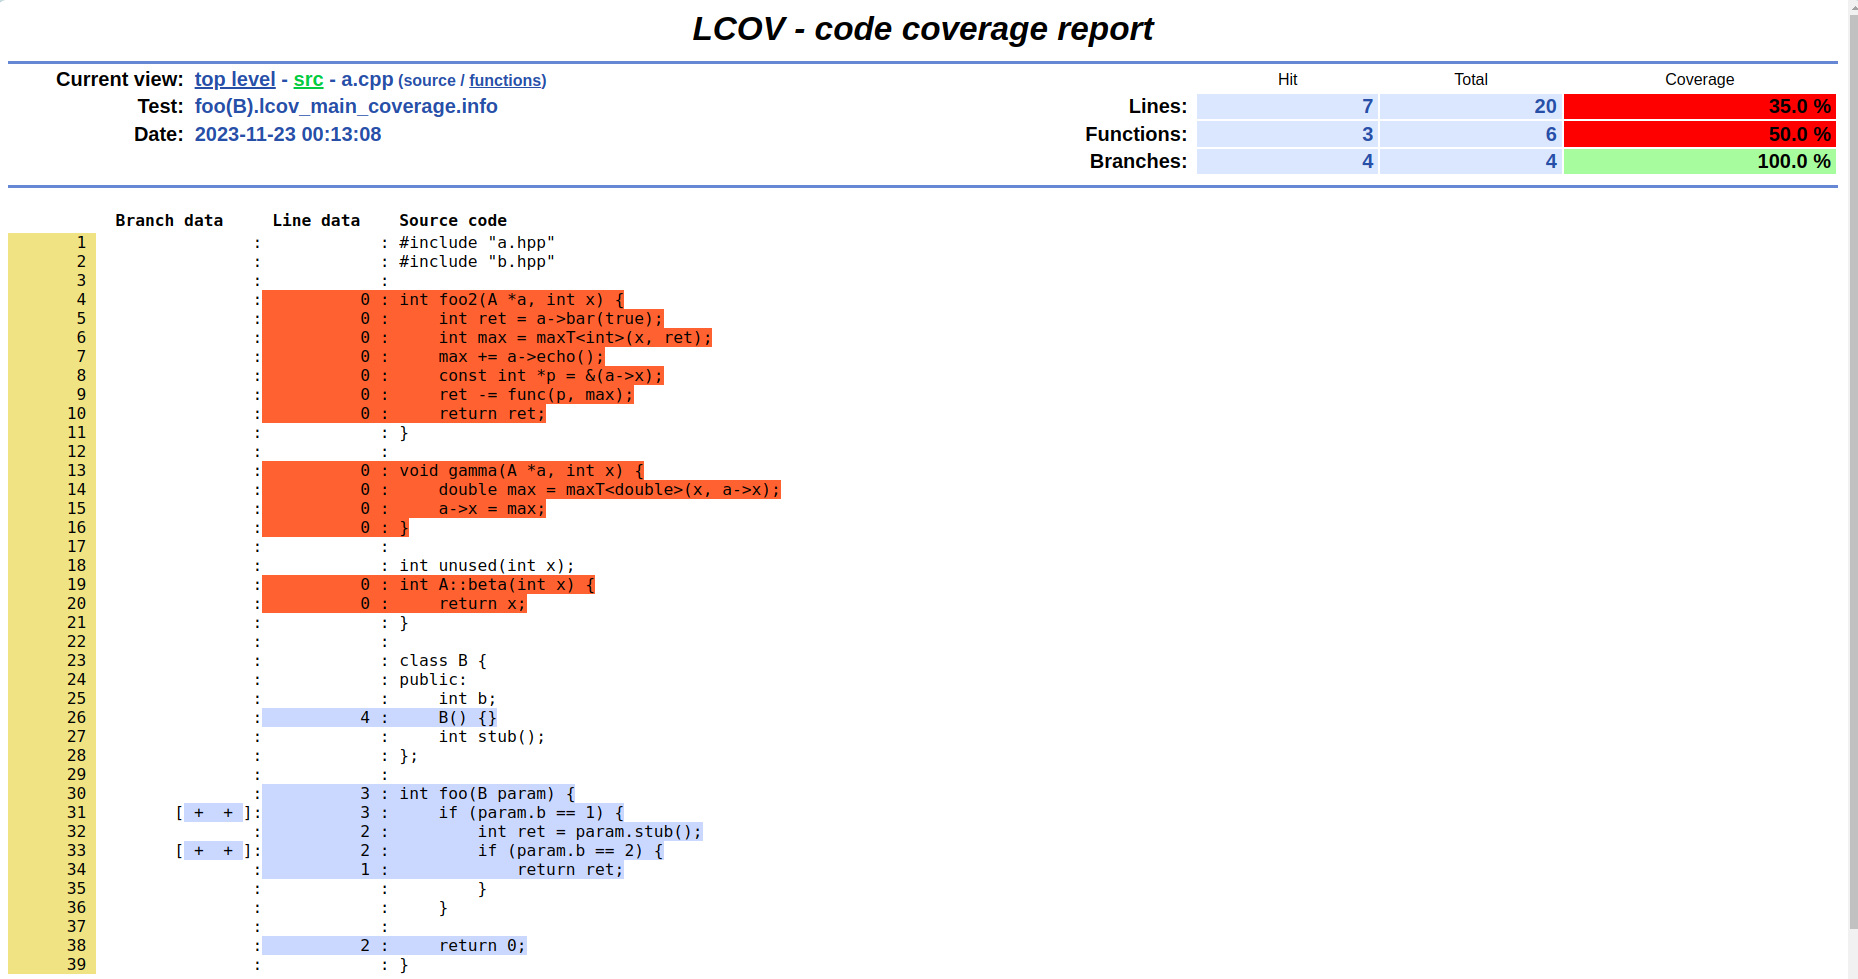
\includegraphics[width=\linewidth]{images/report.png}
    \caption{Báo cáo kiểm thử LCOV của hàm \tcode{foo}.}
    \label{fig:report}
\end{figure}

% \begin{figure}
%     \centering
%     \includesvg[width=0.8\linewidth]{images/module-build.svg}
%     \caption{Các thành phần trong mô-đun xây dựng môi trường kiểm thử.}
%     \label{fig:module-build}
% \end{figure}

% Đầu vào của mô-đun xây dựng môi trường kiểm thử gồm tập mã nguồn kiểm thử và tệp cấu hình kiểm thử được người dùng thiết lập thông qua giao diện của công cụ. Đoạn~mã~\ref{cod:enviro} minh họa tệp cấu hình kiểm thử đầu vào. Dòng 2-11 trong đoạn mã cho biết môi trường kiểm thử sử dụng trình biên dịch GNU mặc định của máy kèm theo một số câu lệnh cơ bản để biên dịch mã nguồn kiểm thử. Dòng 12-14 cho biết thêm thông tin về tên của môi trường kiểm thử, phương pháp kiểm thử cũng như loại độ phủ sẽ được tính là gì. Môi trường ví dụ có tên là \tcode{auto-sample}, sử dụng phương pháp kiểm thử tự động đề xuất bởi khóa luận và hai kiểu độ phủ được tính là độ phủ câu lệnh và độ phủ MCDC. Tệp cấu hình kiểm thử được lưu lại nhằm phục vụ cho các lần kiểm thử sau trên cùng môi trường \tcode{auto-sample}. 
% \begin{figure}[h]
% \begin{lstlisting}[language={}, caption={Tệp cấu hình kiểm thử.}, captionpos=b, label={cod:enviro}]
% ENVIRO.NEW
% ENVIRO.COMPILER.NEW
% ENVIRO.COMPILER.NAME: [GNU Native] C++
% ENVIRO.COMPILER.COMPILE_CMD: g++ -c -w
% ENVIRO.COMPILER.PREPROCESS_CMD: g++ -c -E
% ENVIRO.COMPILER.LINK_CMD: g++ -w
% ENVIRO.COMPILER.INCLUDE_FLAG: -I
% ENVIRO.COMPILER.DEFINE_FLAG: -D
% ENVIRO.COMPILER.OUTPUT_FLAG: -o
% ENVIRO.COMPILER.OUTPUT_EXT: .out
% ENVIRO.COMPILER.END
% ENVIRO.NAME: auto_sample
% ENVIRO.TESTING_METHOD: PROPOSED-METHOD
% ENVIRO.COVERAGE_TYPE: STATEMENT+MCDC
% ENVIRO.END
% \end{lstlisting}
% \end{figure}
\subsection{Mô-đun phân tích mã nguồn}\label{sec:module-analyze}
Mô-đun phân tích mã nguồn đảm nhiệm vai trò trích xuất, phân tích thông tin từ AST của mã nguồn kiểm thử, xây dựng đồ thị cấu trúc mã nguồn và cung cấp dịch vụ tìm kiếm thông tin đỉnh trên đồ thị. Hình~\ref{fig:module-analyze} mô tả cấu trúc của mô-đun với ba thành phần lần lượt là thành phần sinh AST, thành phần sinh đồ thị cấu trúc mã nguồn và thành phần tìm kiếm trên đồ thị. Trong đó, khóa luận kế thừa thành phần sinh AST, cải tiến mô-đun sinh đồ thị cấu trúc mã nguồn và bổ sung thành phần tìm kiếm trên đồ thị.
\vspace{5mm}
\begin{figure}[h]
    \centering
    \includesvg[width=0.8\linewidth]{images/module-analyze.svg}
    \caption{Các thành phần trong mô-đun phân tích mã nguồn.}
    \label{fig:module-analyze}
\end{figure}

Mô-đun phân tích mã nguồn nhận đầu vào là mã nguồn kiểm thử gốc và các đỉnh tệp từ đầu ra của mô-đun xây dựng môi trường. Bắt đầu từ mỗi đỉnh tệp, dựa trên quan hệ cha con trên AST của từng tệp mã nguồn, quá trình sinh cây cấu trúc tệp được diễn ra song song. Sau đó, tập cây cấu trúc tệp được chuyển sang thành phần hoàn thiện đồ thị cấu trúc để bổ sung cạnh kế thừa và cạnh lời gọi hàm. Tại thành phần này, từng cây cấu trúc tệp được xét và tìm kiếm các đỉnh có tiêu chí phù hợp với kiểu cạnh đang xét trên các cây cấu trúc còn lại. Kết quả của quá trình xây dựng là đồ thị cấu trúc mã nguồn kiểm thử.

Khóa luận đã cải tiến thành phần sinh đồ thị cấu trúc mã nguồn như sau. Trước hết, khóa luận tích hợp thành phần ánh xạ cây cấu trúc và thành phần phân tích phụ thuộc~\cite{TUNG2022106821} trong kiến trúc gốc thành mô-đun sinh đồ thị cấu trúc mã nguồn. Quá trình tích hợp bổ sung các luồng xử lý song song quá trình sinh cây cấu trúc tệp giúp giảm thời gian phân tích mã nguồn. Sau đó, khóa luận bổ sung các loại đỉnh mới biểu thị cho các kiểu khai báo mới trong ngôn ngữ C++ như không gian tên, câu lệnh sử dụng không gian tên, khai báo lớp không cần tên kiểu, v.v. Qua đó, thành phần này có thể phân tích và biểu diễn được các đặc trưng mới của C++ trên đồ thị cấu trúc mã nguồn.\\

Tìm kiếm thông tin đỉnh trên đồ thị là quá trình cốt lõi phục vụ cho quá trình xử lý hàm thiếu định nghĩa và quá trình sinh dữ liệu kiểm thử tự động. Trong kiến trúc gốc, quá trình tìm kiếm duyệt qua các đỉnh trên đồ thị, kiểm tra thông tin của đỉnh có hợp với tiêu chí tìm kiếm rồi thêm vào tập kết quả nếu hợp lệ. Trong thực tế, đồ thị cấu trúc thường rất lớn. Vậy nên quá trình tìm kiếm tốn nhiều bộ nhớ bởi quá trình đệ quy xuống đỉnh. Để khắc phục nhược điểm này, khóa luận bổ sung thành phần tìm kiếm trên đồ thị với ý tưởng chính dựa trên tìm kiếm kết hợp bảng băm và cơ sở dữ liệu. Việc tìm kiếm thông tin đỉnh thường sử dụng hai tiêu chí đó là tên hàm và tên kiểu. Tận dụng điều này, khóa luận tạo cơ sở dữ liệu lưu trữ thông tin về kiểu và hàm của mã nguồn kiểm thử. Cơ sở dữ liệu gồm hai trường chính đó là $id$ - khóa chính biểu thị mã định danh của hàm hoặc kiểu và $name$ - tên hàm hoặc tên kiểu. Sau quá trình xây dựng đồ thị cấu trúc mã nguồn, mỗi đỉnh trong đồ thị được cấp một mã định danh cố định $id$. Mã định danh này là giá trị băm xâu đường dẫn của đỉnh, trong đó xâu đường dẫn là chuỗi tên các đỉnh trên đường đi từ đỉnh tệp xuống đỉnh đang xét. Khóa luận sử dụng một bảng băm để ánh xạ $id$ và đỉnh sở hữu $id$. Để nhanh chóng tìm kiếm tên trong cơ sở dữ liệu, khóa luận sử dụng hệ quản trị cơ sở dữ liệu SQLite\footnote{https://www.sqlitetutorial.net/sqlite-full-text-search/} với cơ chế FULLTEXT INDEX trên cột $name$. Để tìm kiếm một đỉnh phù hợp, trước hết quá trình tìm kiếm sẽ thu thập các dòng trong cơ sở dữ liệu có chứa tên hàm hoặc tên kiểu, trích xuất $id$ và dựa vào bảng băm để lấy ra đỉnh cần xét. 

Quá trình nghiên cứu, cải tiến mô-đun phân tích mã nguồn tốn nhiều thời gian do số lượng tệp ảnh hưởng bởi mô-đun này là rất lớn (113 tệp ảnh hưởng và 5476 LOC thay đổi). Tuy nhiên, quá trình trên là cần thiết bởi công cụ AKAUTAUTO phiên bản 5.9.2 thường gặp lỗi hết bộ nhớ ảo trong quá trình phân tích mã nguồn khi chạy trên các dự án có kích thước lớn, cấu trúc phức tạp và có nhiều sự tương tác trong các thành phần với nhau. Sau quá trình cải tiến, công cụ AKAUTAUTO phiên bản 5.9.2-thesis đã có thể phân tích được những bộ mã nguồn có kích thước lớn, đồng thời không gặp tình trạng hết bộ nhớ ảo trong quá trình chạy.

\subsection{Mô-đun xử lý hàm thiếu định nghĩa}\label{sec:module-undef}
Mô-đun xử lý hàm thiếu định nghĩa được khóa luận bổ sung so với kiến trúc gốc nhằm thực hiện nhiệm vụ của pha xử lý hàm thiếu định nghĩa. Hình~\ref{fig:module-undef} mô tả các thành phần cấu thành lên mô-đun gồm thành phần thu thập, thành phần lọc tìm ứng viên, thành phần xử lý nguyên mẫu hàm ảo và thành phần sinh thân hàm giả. Mô-đun xử lý hàm thiếu định nghĩa được thiết kế để xử lý hai loại nguyên mẫu hàm thiếu định nghĩa như đã mô tả ở Mục~\ref{sec:handle-undef}. Chi tiết về các thành phần như sau.
\begin{itemize}
    \item Thành phần thu thập: Đóng vai trò thu thập danh sách các nguyên mẫu hàm thiếu định nghĩa cần sinh thân hàm giả. Thành phần thu thập sử dụng các công cụ tiện ích của trình biên dịch để thu thập danh sách này. Phương pháp thu thập đã được trình bày ở Mục~\ref{sec:handle-undef-first}.
    \item Thành phần xử lý nguyên mẫu hàm ảo: Có chức năng tìm kiếm các nguyên mẫu hàm ảo thiếu định nghĩa sử dụng phương pháp đề xuất ở Mục~\ref{sec:handle-undef-second}. Danh sách các nguyên mẫu hàm ảo tìm được sẽ được truyền sang thành phần lọc tìm ứng viên để xử lý theo Thuật~toán~\ref{alg:handle-virtual-undef}. Các nguyên mẫu hàm ảo còn lại sẽ được sinh cạnh định nghĩa tương ứng với đỉnh biểu thị hàm trong đồ thị cấu trúc.
    \item Thành phần lọc tìm ứng viên: Thực hiện quá trình áp dụng Thuật~toán~\ref{alg:filter-undef} trên danh sách các hàm thiếu định nghĩa trả về bởi thành phần thu thập và các nguyên mẫu hàm ảo thiếu định nghĩa tìm được. Đầu ra của thành phần là danh sách các đỉnh trên đồ thị cấu trúc mã nguồn cần được sinh hàm giả. 
    \item Thành phần sinh thân hàm giả: Đảm nhiệm vai trò sinh thân hàm giả cho danh sách các đỉnh được tổng hợp bởi thành phần lọc tìm ứng viên.
\end{itemize}

\begin{figure}[h]
    \centering
    \includesvg[width=0.8\linewidth]{images/module-undef.svg}
    \caption{Các thành phần trong mô-đun xử lý hàm thiếu định nghĩa.}
    \label{fig:module-undef}
\end{figure}

Đầu ra của mô-đun xử lý hàm thiếu định nghĩa là mã nguồn chứa các câu lệnh đánh dấu đã được bổ sung thân hàm giả cho các nguyên mẫu hàm thiếu định nghĩa. Mã nguồn đã chỉnh sửa này sau đó được sử dụng để tính toán độ phủ khi chạy các ca kiểm thử bởi mô-đun thực thi và phân tích ca kiểm thử.

\subsection{Mô-đun sinh dữ liệu kiểm thử}\label{sec:module-autogen}
Mục tiêu của mô-đun sinh dữ liệu kiểm thử là tự động tạo ra các ca kiểm thử cho các đơn vị cần kiểm thử. Mô-đun được thiết kế như Hình~\ref{fig:module-autogen} với bốn thành phần lần lượt là thành phần sinh CFG, thành phần sinh dữ liệu kiểm thử ngẫu nhiên, thành phần thực thi tượng trưng và thành phần xử lý lời gọi hàm. Trong đó, thành phần xử lý lời gọi hàm được cải tiến bởi phương pháp đề xuất ở Mục \ref{sec:autostub-obj}, các thành phần còn lại được kế thừa từ kiến trúc gốc. Chi tiết về các thành phần như sau.
\begin{itemize}
    \item Thành phần sinh CFG: Có chức năng xây dựng CFG cho các đơn vị trong mã nguồn.
    \item Thành phần sinh dữ liệu kiểm thử ngẫu nhiên: Đảm nhiệm vai trò sinh các ca kiểm thử với dữ liệu ngẫu nhiên trong pha sinh dữ liệu kiểm thử tự động (mô tả ở Mục~\ref{sec:autogen}). 
    \item Thành phần thực thi tượng trưng: Đóng vai trò thực hiện quá trình thực thi tượng trưng trên đường thi hành chưa được viếng thăm và sinh ra các ràng buộc tạo các điểm quyết định trong đồ thị dòng điều khiển. Sau đó, thành phần thực thi tượng trưng sử dụng bộ giải Z3 để giải các ràng buộc và tạo ra các giá trị đầu vào mới.
    \item Thành phần xử lý lời gọi hàm: Có nhiệm vụ tạo giả lập mã nguồn tự động cho các lời gọi hàm xuất hiện trong đường thi hành. Khóa luận kế thừa thành phần xử lý lời gọi hàm dựa trên phương pháp AS4UT và áp dụng phương pháp xử lý lời gọi phương thức được đề xuất ở Mục \ref{sec:autostub-obj}. Đầu ra của thành phần là các thay đổi cần thiết trên CFG, bảng $MAP$ và $REF$ để giúp quá trình thực thi tượng trưng sinh ra bộ dữ liệu kiểm thử mới cho đường thi hành chưa viếng thăm.
\end{itemize}

\begin{figure}[h]
    \centering
    \includesvg[width=0.6\linewidth]{images/module-autogen.svg}
    \caption{Các thành phần trong mô-đun sinh dữ liệu kiểm thử.}
    \label{fig:module-autogen}
\end{figure}
% \subsection{Mô-đun thực thi và phân tích ca kiểm thử}
% \begin{figure}
%     \centering
%     \includesvg[width=0.8\linewidth]{images/module-execute.svg}
%     \caption{Các thành phần trong mô-đun thực thi và phân tích ca kiểm thử.}
%     \label{fig:module-execute}
% \end{figure}

% Đoạn mã \ref{cod:driver} minh họa ví dụ trình điều khiển kiểm thử sinh bởi mô-đun khi kiểm thử hàm \tcode{foo} trong Đoạn~mã~\ref{cod:autostub-object}. Dòng đầu tiên trong trình điều khiển dùng để thiết lập tên đơn vị kiểm thử, giúp các hàm được stub biết cần phải chạy mã nguồn giả lập nào (mô tả trong Đoạn~mã~\ref{cod:stub-final}). Dòng 2-3 định nghĩa tham số đầu vào \tcode{param} của hàm \tcode{foo} là một đối tượng của lớp \tcode{B} với thuộc tính \tcode{b} có giá trị 1. Dòng 4 trong trình điều khiển dùng để gọi hàm \tcode{foo} với các định nghĩa tham số được khai báo ở trên. Kết quả viếng thăm sau quá trình chạy ca kiểm thử được mô tả bởi Đoạn~mã~\ref{cod:visited}. Kết quả viếng thăm cho biết các dòng 8, 9, 10, 11 và nhánh đúng của biểu thức điều kiện ở dòng 8, 10 trong hàm \tcode{foo} được thăm. \\

% \begin{figure}[h]
%     \begin{minipage}[t]{0.5\linewidth}
%     \begin{lstlisting}[language={C++}, caption={Trình điều khiển kiểm thử cho Đoạn mã \ref{cod:autostub-object}.}, captionpos=b, label={cod:driver}]
% TEST_CASE_NAME = "foo";
% B param;
% param.b = 1;
% int AKA_ACTUAL_OUTPUT = foo(param);
%     \end{lstlisting}
%     \end{minipage}
%     \begin{minipage}[t]{0.5\linewidth}
%     \begin{lstlisting}[language=C++, caption={Danh sách các câu lệnh và nhánh điều kiện được thăm bởi trình điều khiển.}, label={cod:visited}, captionpos=b]
% visit_line_8
% visit_condition_1_T
% visit_line_9
% visit_line_10
% visit_condition_1_T
% visit_line_11
%     \end{lstlisting}
% \end{minipage}
% \end{figure}

\section{Mục tiêu, độ đo đánh giá và dữ liệu thực nghiệm}
Mục tiêu tổ chức thực nghiệm là để đánh giá tính hiệu quả của phương pháp đề xuất trên hai tiêu chí với các độ đo tương ứng như sau:
\begin{enumerate}
    \item Đánh giá tính hiệu quả trong quá trình chuẩn bị môi trường kiểm thử cho mã nguồn thiếu định nghĩa giữa phương pháp xử lý hàm thiếu định nghĩa (trình bày ở Mục~\ref{sec:handle-undef}) và phương pháp truyền thống. Để so sánh giữa hai phương pháp, khóa luận sử dụng độ đo thời gian cần thiết để chuẩn bị môi trường kiểm thử. Ngoài ra, khóa luận cũng xem xét tính đúng đắn của phương pháp đề xuất.
    \item Đánh giá tính hiệu quả khi sinh dữ liệu kiểm thử tự động cho một số mã nguồn C/C++ giữa phương pháp đề xuất ở Mục~\ref{sec:autostub-obj} và phương pháp hiện tại trong công cụ phiên bản 5.9.2 - phương pháp kiểm thử tượng trưng động kết hợp tự động giả lập mã nguồn AS4UT (gọi tắt là phương pháp AKAUTAUTO). Để so sánh giữa hai phương pháp, khóa luận sử dụng các độ đo về độ phủ mã nguồn $C_1$, $C_3$, số lượng ca kiểm thử sinh ra, thời gian sinh và bộ nhớ sử dụng trung bình cho mỗi ca kiểm thử.
\end{enumerate}

Về môi trường thực nghiệm, khóa luận sử dụng máy tính với các thông số cấu hình như sau: Ubuntu 22.04, AMD® Ryzen™ 7-5800H CPU @ 3.2GHz x 8, 16GBs RAM. Thực nghiệm được tiến hành trên một số mã nguồn mở trên Github và mã nguồn dự án thực tế thuộc đơn vị FPT-GAM như sau:
\begin{itemize}
    \item C-plus-plus\footnote{https://github.com/TheAlgorithms/C-Plus-Plus} (42179 LOC): Mã nguồn mở viết bằng ngôn ngữ C++ cài đặt các thuật toán thường sử dụng trong lập trình thi đấu và khoa học máy tính.
    \item Box2d\footnote{https://github.com/erincatto/box2d} (78811 LOC): Một thư viện cung cấp các phương thức để tính toán sự tương tác vật lý giữa các vật thể trong môi trường 2 chiều.
    \item FPT1 (23024 LOC): Mô-đun vận hành và điều hướng các yêu cầu gửi đến các dịch vụ trong trình điều khiển đa phương tiện, thuộc một dự án phát triển phần mềm xe ô tô của đơn vị FPT-GAM.
    \item FPT2 (35891 LOC): Mô-đun cung cấp dịch vụ quản lý danh bạ, cuộc gọi trên trình điều khiển đa phương tiện, cũng thuộc dự án trên.
\end{itemize}

Khóa luận sử dụng hai dự án mã nguồn mở nhằm đảm bảo tính khách quan của thực nghiệm. Trong đó, dự án C-plus-plus được sử dụng để đánh giá khả năng sinh dữ liệu kiểm thử của phương pháp đề xuất trên các mã nguồn đơn giản, ít sự liên kết giữa các tệp. Dự án Box2d được chọn để đánh giá tính hiệu quả của phương pháp đề xuất trên các mã nguồn sử dụng nhiều đặc trưng mới của C++. Thêm vào đó, khóa luận cũng sử dụng hai mã nguồn thuộc đơn vị FPT-GAM nhằm đồng thời đánh giá tính hiệu quả và khả năng áp dụng thực tiễn của phương pháp đề xuất.

\section{Đánh giá khả năng xử lý hàm thiếu định nghĩa}
\subsection{Cách thức tổ chức thực nghiệm}
Nhằm đánh giá tính hiệu quả về mặt thời gian khi xử lý hàm thiếu định nghĩa, đồng thời đảm bảo tính khách quan của thực nghiệm, quá trình thực nghiệm được tiến hành bởi lập trình viên\footnote{Trần Trọng Năm - namtt25@fpt.com} trực thuộc đơn vị FPT-GAM. Để mô phỏng môi trường chứa hàm thiếu định nghĩa, khóa luận tiến hành thực nghiệm tính toán thời gian cần thiết để chuẩn bị môi trường kiểm thử cho một số mô-đun trong các mã nguồn mở kể trên. Ba mô-đun thực nghiệm gồm mô-đun collision (xử lý va chạm) trong mã nguồn Box2d, mô-đun FPT1 và mô-đun FPT2. Do mã nguồn C-plus-plus gồm các tệp mã nguồn không liên quan đến nhau nên khóa luận không đánh giá khả năng xử lý hàm thiếu định nghĩa trên mã nguồn này.

Chuẩn bị môi trường kiểm thử là bước đầu tiên trong quy trình kiểm thử tự động. Trong bước này, lập trình viên cần bóc tách mã nguồn mình cần kiểm thử trong dự án và chỉnh sửa mã nguồn sao cho ta có thể tạo được tệp thực thi từ mã nguồn. Để tạo được tệp thực thi, lập trình viên cần xác định các kiểu dữ liệu và các hàm được sử dụng trong mã nguồn mà nằm ở mô-đun khác rồi xử lý các thành phần này để biên dịch được mã nguồn. Sau đó, lập trình viên cần xử lý các hàm thiếu định nghĩa phát sinh do mô-đun chưa phát triển xong để liên kết được các tệp và tạo thành tệp thực thi. Khóa luận tiến hành thu thập thời gian lập trình viên chuẩn bị môi trường kiểm thử giữa phương pháp truyền thống (tức làm thủ công các bước) và phương pháp đề xuất (tức làm thủ công hai bước đầu và để công cụ tự động xử lý các hàm thiếu định nghĩa).
\subsection{Kết quả thực nghiệm}
Bảng~\ref{tab:time_undef} trình bày kết quả thực nghiệm trên mô-đun Box2d, FPT1 và FPT2. Các cột trong bảng có ý nghĩa như sau:
\begin{itemize}
    \item "Module": Tên mô-đun được xét.
    \item "File": Số lượng tệp trong mô-đun.
    \item "Undef": Số lượng hàm thiếu định nghĩa sau khi bóc tách mô-đun.
    \item "Compilable": Thời gian cần thiết để bóc tách mô-đun và chỉnh sửa mã nguồn sao cho biên dịch được.
    \item "Linkable": Thời gian cần thiết để xử lý các hàm thiếu định nghĩa sao cho tạo tệp thực thi được. Trong đó, cột "Manual" thể hiện thời gian xử lý thủ công còn cột "Propose" thể hiện thời gian xử lý sử dụng phương pháp đề xuất (tính bằng giây).
\end{itemize}

\begin{table}[h]
    \centering
    \caption{Kết quả thời gian chuẩn bị môi trường trên ba mô-đun thực nghiệm}
    \label{tab:time_undef}
\begin{tabular}{|l|l|l|l|ll|}
\hline
\multicolumn{1}{|c|}{\multirow{2}{*}{\textbf{Module}}} & \multicolumn{1}{c|}{\multirow{2}{*}{\textbf{File}}} & \multicolumn{1}{c|}{\multirow{2}{*}{\textbf{Undef}}} & \multirow{2}{*}{\textbf{Compilable}} & \multicolumn{2}{c|}{\textbf{Linkable}} \\ \cline{5-6} 
\multicolumn{1}{|c|}{}                                 & \multicolumn{1}{c|}{}                               & \multicolumn{1}{c|}{}                                &                                      & \multicolumn{1}{l|}{Manual}  & Propose \\ \hline
collision (Box2d)                                      & 53                                                  & 5                                                    & 0:02:39                              & \multicolumn{1}{l|}{0:08:23} & 0:00:04 \\ \hline
FPT1                                     & 45                                                  & 263                                                  & 1:04:22                              & \multicolumn{1}{l|}{0:14:48} & 0:00:28 \\ \hline
FPT2                                          & 126                                                 & 333                                                  & 2:05:56                              & \multicolumn{1}{l|}{1:31:01} & 0:02:24 \\ \hline
\end{tabular}
\end{table}

Kết quả thực nghiệm cho thấy thời gian xử lý các hàm thiếu định nghĩa thủ công chiếm một phần đáng kể trong tổng thời gian chuẩn bị môi trường, trong đó thời gian xử lý trên mô-đun collision là 75,98\%, 18,70\% với mô-đun FPT1 và 41,96\% với mô-đun còn lại. Khi áp dụng phương pháp đề xuất, thời gian xử lý các hàm thiếu định nghĩa giảm đáng kể so với phương pháp truyền thống, giảm 8 phút 19 giây trên mô-đun collision, 14 phút 20 giây trên mô-đun FPT1 và giảm 1 tiếng 29 phút trên mô-đun còn lại. Dựa vào kết quả, có thể nhận thấy rằng thời gian xử lý của hai phương pháp phụ thuộc vào số lượng hàm thiếu định nghĩa có trong mô-đun.

\subsection{Đánh giá}
Kết quả thực nghiệm cho thấy rằng phương pháp đề xuất có khả năng giảm đáng kể thời gian chuẩn bị môi trường kiểm thử cho mã nguồn chứa hàm thiếu dịnh nghĩa. Một số lí do chính dẫn đến sự cải thiện đáng kể này như sau:
\begin{itemize}
    \item Trước hết, thời gian xử lý thủ công bị ảnh hưởng bởi kích thước và độ phức tạp của mã nguồn. Các mô-đun có thể phụ thuộc bởi rất nhiều mô-đun khác và đồng thời chúng cũng chứa rất nhiều tệp. Điều này gây khó khăn cho lập trình viên khi họ cần xác định vị trí các tệp chứa hàm thiếu định nghĩa. Phương pháp đề xuất chỉ quan tâm tới danh sách các hàm trả về bởi trình biên dịch và kết hợp duyệt trên đồ thị cấu trúc mã nguồn nên nhanh chóng xác định và xử lý đúng hàm thiếu định nghĩa.
    \item Quá trình xử lý hàm thiếu định nghĩa thủ công đòi hỏi lập trình viên có kiến thức về mã nguồn kiểm thử. Điều này khiến lập trình viên tốn nhiều thời gian để nghiên cứu mã nguồn và xử lý chính xác các hàm thiếu định nghĩa. Trong bối cảnh ngôn ngữ C++ đang được phát triển với nhiều đặc trưng mới ra mắt, việc xử lý thủ công có thể tiêu tốn nhiều chi phí về nhân lực và thời gian hơn.
    \item Cuối cùng, phương pháp đề xuất có thể xử lý song song các hàm trong khi lập trình viên cần xử lý tuần tự từng hàm. Điều này dẫn tới thời gian xử lý giảm đáng kể so với phương pháp truyền thống.
\end{itemize}

Để đánh giá tính đúng đắn của phương pháp đề xuất, khóa luận đã tiến hành thực nghiệm sinh dữ liệu kiểm thử tự động cho các đơn vị trong mã nguồn sau khi xử lý hàm thiếu định nghĩa (trình bày ở Mục~\ref{sec:evaluate-autogen}). Kết quả cho thấy các ca kiểm thử đều thực thi được và không gặp lỗi trong quá trình liên kết. Như vậy, phương pháp đề xuất đã xử lý đúng và đủ các hàm thiếu định nghĩa cần thiết. Điều này được khẳng định bởi nếu phương pháp xử lý thiếu hoặc sai hàm, mã nguồn kiểm thử không thể liên kết và thực thi các ca kiểm thử được. Tính đến thời điểm nghiên cứu của khóa luận, phương pháp đề xuất đã giải quyết được các mã nguồn thực nghiệm chứa các đặc trưng của ngôn ngữ C++ ở nhiều phiên bản, mới nhất là bản C++20. Tuy nhiên trong các phiên bản tương lai, tính đúng đắn của phương pháp đề xuất có thể bị ảnh hưởng.

Như vậy, phương pháp đề xuất có thể áp dụng vào thực tiễn để giúp giảm thời gian kiểm thử đơn vị tự động. Tuy nhiên, có thể nhận thấy rằng thấy phương pháp đề xuất vẫn còn phụ thuộc vào bước bóc tách mã nguồn và xử lý sao cho biên dịch được. Việc phụ thuộc vào các bước thủ công khiến quá trình chuẩn bị môi trường kiểm thử tốn nhiều thời gian, đặc biệt là khi kiểm thử cho mã nguồn kích thước lớn. Một số lí do dẫn đến phương pháp chưa hoàn toàn tự động được như sau:
\begin{itemize}
    \item Quá trình bóc tách mã nguồn yêu cầu công cụ trích xuất được đúng các tệp có liên quan đến mô-đun người dùng mong muốn kiểm thử. Điều này gây khó khăn bởi để trích xuất được chính xác mô-đun, công cụ cần phân tích mã nguồn của cả dự án để biết được các quan hệ giữa mô-đun và các thành phần khác. Việc phân tích mã nguồn dự án tốn nhiều thời gian và có thể cần phân tích nhiều lần do quá trình phát triển song song với quá trình kiểm thử.
    \item Quá trình tự động xử lý các kiểu dữ liệu và các hàm ở mô-đun khác sao cho biên dịch được mã nguồn có thể không chính xác. Khi kiểm thử, ta muốn hạn chế sự tác động đến mã nguồn gốc. Do vậy, các kiểu dữ liệu và hàm ở mô-đun khác thường được sao chép ở một tệp và mô-đun kiểm thử sẽ sử dụng tệp sao chép này. Khi tự động hóa quá trình này, công cụ cần phân tích mã nguồn để biết chính xác nên sao chép kiểu nào, hàm nào và vị trí ở đâu.
\end{itemize}
 
\section{Đánh giá khả năng sinh dữ liệu kiểm thử tự động}\label{sec:evaluate-autogen}
\subsection{Cách thức tổ chức thực nghiệm}
Nhằm đánh giá tính hiệu quả khi sinh dữ liệu kiểm thử tự động, khóa luận tiến hành thực nghiệm trên công cụ AKAUTAUTO phiên bản 5.9.2, được cài đặt phương pháp kiểm thử tượng trưng động AKAUTAUTO và phương pháp AS4UT, và phiên bản 5.9.2-thesis, được cài đặt phương pháp đề xuất. Các mã nguồn được sử dụng trong thực nghiệm này gồm mã nguồn C-plus-plus, mã nguồn Box2d và mã nguồn FPT1. Khóa luận chưa thể đánh giá khả năng sinh dữ liệu kiểm thử tự động trên mã nguồn FPT2 do mã nguồn này được bảo mật bởi đơn vị FPT-GAM.

\subsection{Kết quả thực nghiệm}
Bảng \ref{tab:autogen-result} trình bày kết quả thực nghiệm sinh dữ liệu kiểm thử tự động cho một số tệp trong các mã nguồn C-plus-plus, Box2d và FPT1 giữa phương pháp AKAUTAUTO và phương pháp đề xuất. Trong đó, bốn tệp đầu được lấy từ dự án C-plus-plus, ba tệp tiếp theo được lấy từ dự án Box2d và năm tệp còn lại từ mô-đun FPT1. Các cột trong bảng có ý nghĩa như sau:
\begin{itemize}
    \item "File": Tên tệp mã nguồn đuôi .cpp được kiểm thử.
    \item "Unit": Số lượng hàm trong tệp mã nguồn được kiểm thử.
    \item "C1": Độ phủ $C_1$ của tệp mã nguồn.
    \item "C3": Độ phủ $C_3$ của tệp mã nguồn.
    \item "Num": Số lượng ca kiểm thử cần thiết để đạt được độ phủ tương ứng.
    \item "Mem": Bộ nhớ sử dụng trung bình (KB) khi sinh dữ liệu kiểm thử tự động cho một hàm trong tệp.
    \item "Time": Thời gian sinh trung bình (giây) khi sinh dữ liệu kiểm thử tự động cho một hàm trong tệp.
\end{itemize}

\begin{table}[h]
    \centering
    \caption{Kết quả thực nghiệm sinh dữ liệu kiểm thử tự động cho một số mã nguồn}
    \label{tab:autogen-result}
\resizebox{\textwidth}{!}{%
\begin{tabular}{|l|l|lllll|lllll|}
\hline
\multicolumn{1}{|c|}{\multirow{2}{*}{\textbf{File}}} & \multicolumn{1}{c|}{\multirow{2}{*}{\textbf{Unit}}} & \multicolumn{5}{c|}{\textbf{AKAUTAUTO Current Method}}                                                                                              & \multicolumn{5}{c|}{\textbf{Proposed Method}}                                                                                                                   \\ \cline{3-12} 
\multicolumn{1}{|c|}{}                               & \multicolumn{1}{c|}{}                               & \multicolumn{1}{c|}{C1}    & \multicolumn{1}{c|}{C3}    & \multicolumn{1}{c|}{Num} & \multicolumn{1}{c|}{Mem}     & \multicolumn{1}{c|}{Time} & \multicolumn{1}{c|}{C1}             & \multicolumn{1}{c|}{C3}             & \multicolumn{1}{c|}{Num} & \multicolumn{1}{c|}{Mem}     & \multicolumn{1}{c|}{Time} \\ \hline
avltree.cpp                                          & 10                                                  & \multicolumn{1}{l|}{91}    & \multicolumn{1}{l|}{80.55} & \multicolumn{1}{l|}{38}  & \multicolumn{1}{l|}{1856.31} & 4.42                      & \multicolumn{1}{l|}{\textbf{99.29}} & \multicolumn{1}{l|}{\textbf{100}}   & \multicolumn{1}{l|}{25}  & \multicolumn{1}{l|}{1299.69} & 4.73                      \\ \hline
binary\_search\_tree.cpp                             & 9                                                   & \multicolumn{1}{l|}{100}   & \multicolumn{1}{l|}{100}   & \multicolumn{1}{l|}{24}  & \multicolumn{1}{l|}{1048.37} & 5.61                      & \multicolumn{1}{l|}{\textbf{100}}   & \multicolumn{1}{l|}{\textbf{100}}   & \multicolumn{1}{l|}{42}  & \multicolumn{1}{l|}{870.71}  & 10.90                     \\ \hline
binaryheap.cpp                                       & 11                                                  & \multicolumn{1}{l|}{77.22} & \multicolumn{1}{l|}{24.16} & \multicolumn{1}{l|}{47}  & \multicolumn{1}{l|}{357.88}  & 2.51                      & \multicolumn{1}{l|}{\textbf{94.34}} & \multicolumn{1}{l|}{\textbf{73.75}} & \multicolumn{1}{l|}{46}  & \multicolumn{1}{l|}{238.66}  & 8.32                      \\ \hline
double\_linked\_list.cpp                             & 6                                                   & \multicolumn{1}{l|}{54.44} & \multicolumn{1}{l|}{31.66} & \multicolumn{1}{l|}{15}  & \multicolumn{1}{l|}{3269.37} & 4.43                      & \multicolumn{1}{l|}{\textbf{54.44}} & \multicolumn{1}{l|}{\textbf{31.66}} & \multicolumn{1}{l|}{34}  & \multicolumn{1}{l|}{405.41}  & 14.94                     \\ \hline
b2\_dynamic\_tree.cpp                                & 12                                                  & \multicolumn{1}{l|}{59.06} & \multicolumn{1}{l|}{45.12} & \multicolumn{1}{l|}{56}  & \multicolumn{1}{l|}{1101.79} & 175.82                    & \multicolumn{1}{l|}{\textbf{72.13}} & \multicolumn{1}{l|}{\textbf{64.32}} & \multicolumn{1}{l|}{37}  & \multicolumn{1}{l|}{295.80}  & 102.15                    \\ \hline
b2\_board\_phase.cpp                                 & 7                                                   & \multicolumn{1}{l|}{49.87} & \multicolumn{1}{l|}{26.85} & \multicolumn{1}{l|}{45}  & \multicolumn{1}{l|}{1611.60} & 206.98                    & \multicolumn{1}{l|}{\textbf{83.81}} & \multicolumn{1}{l|}{\textbf{68.75}} & \multicolumn{1}{l|}{31}  & \multicolumn{1}{l|}{5105.65} & 83.35                     \\ \hline
b2\_collide\_edge.cpp                                & 3                                                   & \multicolumn{1}{l|}{51.85} & \multicolumn{1}{l|}{44}    & \multicolumn{1}{l|}{15}  & \multicolumn{1}{l|}{2611.99} & 91.44                     & \multicolumn{1}{l|}{\textbf{76.44}} & \multicolumn{1}{l|}{\textbf{67.13}} & \multicolumn{1}{l|}{32}  & \multicolumn{1}{l|}{6020.06} & 263.73                    \\ \hline
FPT1\_file1.cpp                                    & 185                                                 & \multicolumn{1}{l|}{89.26} & \multicolumn{1}{l|}{60.67} & \multicolumn{1}{l|}{668} & \multicolumn{1}{l|}{442.53}  & 268.36                    & \multicolumn{1}{l|}{\textbf{98.43}} & \multicolumn{1}{l|}{\textbf{96.05}} & \multicolumn{1}{l|}{703} & \multicolumn{1}{l|}{188.49}  & 46.28                     \\ \hline
FPT1\_file2.cpp                               & 17                                                  & \multicolumn{1}{l|}{46.40} & \multicolumn{1}{l|}{29.29} & \multicolumn{1}{l|}{40}  & \multicolumn{1}{l|}{1353.71} & 54.60                     & \multicolumn{1}{l|}{\textbf{95.41}} & \multicolumn{1}{l|}{\textbf{86.55}} & \multicolumn{1}{l|}{75}  & \multicolumn{1}{l|}{23.79}   & 63.33                     \\ \hline
FPT1\_file3.cpp                                   & 1                                                   & \multicolumn{1}{l|}{66.67} & \multicolumn{1}{l|}{16.67} & \multicolumn{1}{l|}{7}   & \multicolumn{1}{l|}{21.34}   & 72.75                     & \multicolumn{1}{l|}{\textbf{100}}   & \multicolumn{1}{l|}{\textbf{100}}   & \multicolumn{1}{l|}{7}   & \multicolumn{1}{l|}{15.20}   & 54.20                     \\ \hline
FPT1\_file4.cpp                                    & 4                                                   & \multicolumn{1}{l|}{63.07} & \multicolumn{1}{l|}{16.67} & \multicolumn{1}{l|}{13}  & \multicolumn{1}{l|}{108.48}  & 278.04                    & \multicolumn{1}{l|}{\textbf{63.07}} & \multicolumn{1}{l|}{\textbf{16.67}} & \multicolumn{1}{l|}{10}  & \multicolumn{1}{l|}{6.68}    & 21.35                     \\ \hline
FPT1\_file5.cpp                                 & 2                                                   & \multicolumn{1}{l|}{92.86} & \multicolumn{1}{l|}{50}    & \multicolumn{1}{l|}{4}   & \multicolumn{1}{l|}{23.34}   & 10.91                     & \multicolumn{1}{l|}{\textbf{92.86}} & \multicolumn{1}{l|}{\textbf{50}}    & \multicolumn{1}{l|}{4}   & \multicolumn{1}{l|}{4.37}    & 9.36                      \\ \hline
\end{tabular}%
}
\end{table}

Kết quả thực nghiệm ở Bảng \ref{tab:autogen-result} cho thấy phương pháp đề xuất sinh dữ liệu kiểm thử có độ phủ $C_1$, $C_3$ luôn cao hơn hoặc bằng phương pháp AKAUTAUTO trên các tệp mã nguồn được kiểm thử. Trong đó, phương pháp đề xuất đạt độ phủ cao hơn khi kiểm thử cho 2/4 tệp của dự án C-plus-plus, 3/3 tệp của dự án Box2d và 3/5 tệp của dự án FPT1. So sánh độ phủ trung bình giữa hai phương pháp trên các tệp của từng dự án, phương pháp đề xuất có độ phủ trung bình cao hơn và tăng đáng kể khi xét độ phủ $C_3$. Cụ thể, với bốn tệp thuộc dự án C-plus-plus, độ phủ $C_1$, $C_3$ trung bình tăng lần lượt 6.35\% và 17.26\%. Ba tệp của dự án Box2d có độ phủ $C_1$, $C_3$ trung bình tăng lần lượt 23.87\% và 28.08\%. Năm tệp của dự án FPT1 tăng lần lượt 18.30\% và 35.19\% với các độ đo tương ứng.

Về mặt độ phủ $C_1$, $C_3$ đạt được trên từng hàm kiểm thử, kết quả trên ba dự án đều cho thấy phương pháp đề xuất đạt được độ phủ cao hơn hoặc bằng phương pháp AKAUTAUTO. Trước hết, với dự án C-plus-plus, các Hình~\ref{fig:c1-algo}, \ref{fig:c3-algo} cho thấy độ phủ $C_1$, $C_3$ của phương pháp đề xuất đạt 100\% cho hầu hết các hàm trong hai tệp đầu, tăng mạnh độ phủ~$C_3$ cho các hàm trong tệp \tcode{binary\_search\_tree.cpp} và giữ nguyên đối với các hàm trong tệp còn lại. Trên dự án Box2d, Hình~\ref{fig:c1-box2d} và \ref{fig:c3-box2d} cho thấy phương pháp đề xuất có tăng đáng kể độ phủ $C_1$, $C_3$ trên 10/22 đơn vị. Tuy nhiên, phương pháp đề xuất không cải thiện độ phủ trên 12 đơn vị còn lại. Cuối cùng, với dự án FPT1, các Hình~\ref{fig:c1-serviceproxy}, \ref{fig:c3-serviceproxy} cho thấy phương pháp đề xuất tăng độ phủ $C_1$, $C_3$ với phần lớn các đơn vị, trong đó 95/209 đơn vị với độ phủ $C_1$ và 173/209 đơn vị với độ phủ $C_3$. Kết quả chi tiết độ phủ trên từng đơn vị kiểm thử cho thấy rằng đối với các đơn vị đã đạt 100\% bởi phương pháp AKAUTAUTO, phương pháp đề xuất cũng đạt 100\% với các đơn vị đó. Tuy nhiên, kết quả độ phủ của phương pháp AKAUTAUTO cho thấy tuy độ phủ $C_1$ của đơn vị có thể đạt 100\% nhưng các nhánh điều kiện trong đơn vị có thể chưa được kiểm tra hết, dẫn tới độ phủ $C_3$ thấp. 

\begin{figure}[H]
    \centering
    \includesvg[width=\linewidth]{images/cppalgo/c1algo.svg}
    \caption{So sánh độ phủ $C_1$ giữa phương pháp đề xuất và phương pháp AKAUTAUTO trên một số hàm trong C-plus-plus.}
    \label{fig:c1-algo}
\end{figure}

\begin{figure}[H]
    \centering
    \includesvg[width=\linewidth]{images/cppalgo/c3algo.svg}
    \caption{So sánh độ phủ $C_3$ giữa phương pháp đề xuất và phương pháp AKAUTAUTO trên một số hàm trong C-plus-plus.}
    \label{fig:c3-algo}
\end{figure}

\begin{figure}[H]
	\centering
	\includesvg[width=\linewidth]{images/box2d/c1box2d.svg}
	\caption{So sánh độ phủ $C_1$ giữa phương pháp đề xuất và phương pháp AKAUTAUTO trên một số hàm trong Box2d.}
	\label{fig:c1-box2d}
\end{figure}

\begin{figure}[H]
	\centering
	\includesvg[width=\linewidth]{images/box2d/c3box2d.svg}
	\caption{So sánh độ phủ $C_3$ giữa phương pháp đề xuất và phương pháp AKAUTAUTO trên một số hàm trong Box2d.}
	\label{fig:c3-box2d}
\end{figure}

\begin{figure}[H]
	\centering
	\includesvg[width=\linewidth]{images/serviceproxy/c1serviceproxy.svg}
	\caption{So sánh độ phủ $C_1$ giữa phương pháp đề xuất và phương pháp AKAUTAUTO trên các hàm trong mô-đun FPT1.}
	\label{fig:c1-serviceproxy}
\end{figure}

\begin{figure}[H]
	\centering
	\includesvg[width=\linewidth]{images/serviceproxy/c3serviceproxy.svg}
	\caption{So sánh độ phủ $C_3$ giữa phương pháp đề xuất và phương pháp AKAUTAUTO trên các hàm trong mô-đun FPT1.}
	\label{fig:c3-serviceproxy}
\end{figure}

Xét số lượng ca kiểm thử tối thiểu sinh để đạt độ phủ tương ứng của hai phương pháp, có thể nhận thấy rằng số ca kiểm thử tối thiểu phụ thuộc vào từng dự án. Đối với dự án C-plus-plus, Hình~\ref{fig:num-algo} cho thấy rằng với các đơn vị không có quá nhiều sự chênh lệnh về độ phủ, số ca kiểm thử tối thiểu chênh lệch ít. Tuy nhiên, với các đơn vị có sự tăng về độ phủ $C_1$ hoặc $C_3$, số ca kiểm thử tăng trong khoảng 2-6 lần. Đặc điểm tương tự diễn ra khi kiểm thử dự án Box2d (mô tả ở Hình~\ref{fig:num-box2d}). Một số trường hợp đột biến về sự chênh lệnh số ca kiểm thử chủ yếu bởi phương pháp xử lý lời gọi phương thức hoặc đơn vị kiểm thử chứa nhiều vòng lặp. Với dự án FPT1, do mã nguồn chứa nhiều sự tương tác giữa các đối tượng, Hình~\ref{fig:num-serviceproxy} cho thấy phần lớn các đơn vị (164/209) có số lượng ca kiểm thử tối thiểu của phương pháp đề xuất nhiều hơn phương pháp AKAUTAUTO.

\begin{figure}[H]
    \centering
    \includesvg[width=\linewidth]{images/cppalgo/numalgo.svg}
    \caption{So sánh số ca kiểm thử sinh ra giữa phương pháp đề xuất và phương pháp AKAUTAUTO trên một số hàm trong C-plus-plus.}
    \label{fig:num-algo}
    
	\includesvg[width=\linewidth]{./images/box2d/numbox2d.svg}
	\caption{So sánh số ca kiểm thử sinh ra giữa phương pháp đề xuất và phương pháp AKAUTAUTO trên một số hàm trong Box2d.}
	\label{fig:num-box2d}

	\includesvg[width=\linewidth]{images/serviceproxy/numserviceproxy.svg}
	\caption{So sánh số ca kiểm thử sinh ra giữa phương pháp đề xuất và phương pháp AKAUTAUTO trên các hàm trong mô-đun FPT1.}
	\label{fig:num-serviceproxy}
\end{figure}

Về thời gian sinh dữ liệu kiểm thử tự động, kết quả cho thấy có 4/4 tệp của dự án C-plus-plus, 1/3 tệp của dự án Box2d và 1/5 tệp của dự án FPT1 mà phương pháp đề xuất sử dụng nhiều thời gian hơn. Ngược lại, phương pháp đề xuất có thời gian sinh ít hơn phương pháp AKAUTAUTO trên các tệp còn lại. Hình~\ref{fig:time-algo}, \ref{fig:time-box2d} và~\ref{fig:time-serviceproxy} phản ánh thời gian sinh dữ liệu kiểm thử cho các tệp trên từng dự án. Do dự án C-plus-plus không chứa nhiều lời gọi phương thức nên phương pháp đề xuất sử dụng nhiều thời gian hơn trên phần lớn các đơn vị kiểm thử. Với hai dự án còn lại, có thể nhận thấy rằng đa phần phương pháp đề xuất sử dụng ít thời gian hơn. Do dự án Box2d chứa nhiều vòng lặp nên thời gian sử dụng phụ thuộc vào số lượng ca kiểm thử và số lần lặp.

\begin{figure}[H]
    \centering
    \includesvg[width=\linewidth]{images/cppalgo/timealgo.svg}
    \caption{So sánh thời gian chạy giữa phương pháp đề xuất và phương pháp AKAUTAUTO trên một số hàm trong C-plus-plus.}
    \label{fig:time-algo}
\end{figure}

\begin{figure}[H]
	\centering
	\includesvg[width=\linewidth]{images/box2d/timebox2d.svg}
	\caption{So sánh thời gian chạy giữa phương pháp đề xuất và phương pháp AKAUTAUTO trên một số hàm trong Box2d.}
	\label{fig:time-box2d}
\end{figure}

\begin{figure}[H]
	\centering
	\includesvg[width=\linewidth]{images/serviceproxy/timeserviceproxy.svg}
	\caption{So sánh thời gian chạy giữa phương pháp đề xuất và phương pháp AKAUTAUTO trên các hàm trong mô-đun FPT1.}
	\label{fig:time-serviceproxy}
\end{figure}

Về bộ nhớ sử dụng để sinh dữ liệu kiểm thử, phương pháp đề xuất sử dụng ít bộ nhớ hơn trên phần lớn các tệp được kiểm thử (10/12). Các trường hợp sử dụng nhiều bộ nhớ hơn là bởi quá trình thực thi tượng trưng xử lý nhiều vòng lặp và các lời gọi phương thức. Ngoài các trường hợp trên, không có lý do rõ ràng giải thích cho sự khác biệt trong lượng bộ nhớ sử dụng của hai phương pháp.

\begin{figure}[H]
    \centering
    \includesvg[width=\linewidth]{images/cppalgo/memalgo.svg}
    \caption{So sánh bộ nhớ sử dụng ra giữa phương pháp đề xuất và phương pháp AKAUTAUTO trên một số hàm trong C-plus-plus.}
    \label{fig:mem-algo}
\end{figure}

\begin{figure}[H]
    \centering
    \includesvg[width=\linewidth]{images/box2d/membox2d.svg}
    \caption{So sánh bộ nhớ sử dụng ra giữa phương pháp đề xuất và phương pháp AKAUTAUTO trên một số hàm trong Box2d.}
    \label{fig:mem-box2d}
\end{figure}

\begin{figure}[H]
    \centering
    \includesvg[width=\linewidth]{images/serviceproxy/memserviceproxy.svg}
    \caption{So sánh bộ nhớ sử dụng giữa phương pháp đề xuất và phương pháp AKAUTAUTO trên các hàm trong mô-đun FPT1.}
    \label{fig:mem-serviceproxy}
\end{figure}

\subsection{Đánh giá}
Kết quả thực nghiệm cho thấy rằng phương pháp đề xuất hiệu quả hơn về mặt độ phủ mã nguồn so với phương pháp AKAUTAUTO khi sinh dữ liệu kiểm thử tự động, đặc biệt ở độ phủ $C_3$. Một số lí do chính dẫn đến sự cải thiện như sau:
\begin{itemize}
    \item Phương pháp đề xuất kế thừa phương pháp kiểm thử tượng trưng động nên có cùng khả năng sinh dữ liệu tự động cho các kiểu dữ liệu nguyên thủy và tự định nghĩa với phương pháp AKAUTAUTO. Bởi vậy, các dự án không chứa nhiều lời gọi phương thức như C-plus-plus vẫn có thể áp dụng phương pháp đề xuất để sinh dữ liệu kiểm thử.
  
    \item Phương pháp đề xuất kế thừa và cải tiến phương pháp AS4UT nên có khả năng giả lập mã nguồn trả về tự động tương tự như AS4UT. Điều này khiến quá trình thực thi tượng trưng xử lý được các ràng buộc liên quan đến giá trị trả về của lời gọi hàm, giúp tăng độ phủ.
    
    \item Độ phủ mã nguồn có sự tăng đột phá bởi cải tiến trong quá trình xử lý lời gọi hàm. Dự án Box2d và FPT1 được viết trên ngôn ngữ C++, sử dụng nhiều đặc trưng hướng đối tượng và các thành phần trong mã nguồn tương tác với nhau thông qua lời gọi phương thức của đối tượng. Do vậy, mã nguồn chứa nhiều biểu thức điều kiện liên quan đến thuộc tính của các đối tượng. Phương pháp đề xuất đã xử lý các lời gọi phương thức nên quá trình thực thi tượng trưng có thể giải được các điều kiện có liên quan đến đối tượng gọi hàm. Phương pháp AS4UT chỉ xử lý cho kết quả trả về của lời gọi hàm nên quá trình thực thi tượng trưng chưa giải được các điều kiện liên quan đến sự thay đổi giá trị của thuộc tính thông qua lời gọi hàm.
\end{itemize}

Tuy nhiên, có thể nhận thấy rằng một số tệp mã nguồn không tăng kết quả độ phủ so với phương pháp AKAUTAUTO. Điều này được lí giải bởi các nguyên nhân sau:
\begin{itemize}
    \item Đơn vị kiểm thử chứa nhiều kiểu dữ liệu chưa được hỗ trợ bởi phương pháp đề xuất như con trỏ thông minh, kiểu dữ liệu template, v.v. Phương pháp đề xuất chưa phân tích được các câu lệnh, điều kiện chứa các kiểu dữ liệu này nên không thể sinh ra các ràng buộc thỏa mãn các câu lệnh, điều kiện tương ứng.
    
    \item Hạn chế trong việc chuyển đổi các câu lệnh, điều kiện trong mã nguồn trong quá trình thực thi tượng trưng khiến phương pháp không tìm được nghiệm khả thi.
    
    \item Đơn vị kiểm thử không chứa lời gọi phương thức nên phương pháp đề xuất không cải thiện được độ phủ. Đóng góp chính của phương pháp đề xuất trong việc sinh dữ liệu kiểm thử tự động nằm ở việc xử lý các lời gọi phương thức. Vì vậy, đối với các đơn vị không chứa lời gọi phương thức, phương pháp đề xuất sẽ cho ra kết quả giống với phương pháp AKAUTAUTO áp dụng AS4UT.
    
    \item Phương pháp đề xuất chưa xử lý tốt vòng lặp xuất hiện trong đơn vị kiểm thử. Các dự án C++ thường chứa nhiều câu lệnh duyệt phần tử trong các tập hợp như \tcode{vector, set}. Các ràng buộc liên quan đến phép duyệt như vậy chưa được hỗ trợ.
    
    \item Phương pháp đề xuất chưa xử lý được lời gọi hàm trong thư viện khiến quá trình thực thi tượng trưng không giải được ràng buộc liên quan đến kết quả của lời gọi thư viện.
\end{itemize}

Về khía cạnh số lượng ca kiểm thử, phương pháp đề xuất sinh nhiều ca kiểm thử hơn nếu mã nguồn chứa lời gọi phương thức. Nguyên nhân là do phương pháp đề xuất cần sinh thêm ca kiểm thử để phủ được điều kiện nhánh liên quan đến sự thay đổi của đối tượng sau lời gọi phương thức.

Hai khía cạnh cuối cùng mà khóa luận đánh giá đó là thời gian và bộ nhớ sử dụng để sinh dữ liệu kiểm thử. Hai yếu tố này phụ thuộc nhiều vào cấu trúc và độ phức tạp của mã nguồn. Trong đó, thời gian xử lý bị ảnh hưởng bởi quá trình thực thi tượng trưng, tìm kiếm kiểu dữ liệu hợp lý và quá trình sinh bộ tham số đầu vào cho đơn vị kiểm thử. Với các dự án sử dụng nhiều lời gọi phương thức, phương pháp đề xuất sử dụng ít thời gian hơn. Nguyên nhân là bởi phương pháp không mất quá nhiều thời gian để giải một đường đi thi hành chứa lời gọi phương thức. Phương pháp AKAUTAUTO cố gắng tìm nghiệm cho các đường thi hành như vậy nên tiêu thụ nhiều thời gian hơn. Khía cạnh bộ nhớ sử dụng cũng ảnh hưởng bởi các yếu tố tương tự. Tuy nhiên, từ kết quả thực nghiệm, có thể nhận thấy rằng phương pháp đã giải quyết được vấn đề liên quan đến lời gọi phương thức và thể hiện tính khả thi khi áp dụng thực tiễn.
